\documentclass[
	aspectratio=169, % default is 43
	8pt, % font size, default is 11pt
	%handout, % handout mode without animations, comment out to add animations
	%nosectionframes, % disable automatic frames at the begin of each section (default: sectiontitleslides in beamer mode and sectionoverviews in handout mode)
	%sectiontitleslides, % enable an automatic section title slide at the begin of each section
	%sectionoverviews, % enable an automatic section overview at the begin of each section
	%uniqueslidenumber, % will uniquely identify pages with overlays by a little suffix
	%darkmode, % switch to dark mode (do not use for presentation with a projector)
]{beamer}
\usepackage{fancybeamer} % use the fancy beamer package
\usepackage{amsmath}
\usepackage[labelformat=empty]{caption}


% custom environments for literate haskell
\usepackage[outputdir=build]{minted}
\newenvironment{code}{\VerbatimEnvironment\begin{minted}{haskell}}{\end{minted}}
\newenvironment{spec}{\VerbatimEnvironment\begin{minted}{haskell}}{\end{minted}}
\newenvironment{demo}{\VerbatimEnvironment\begin{minted}{haskell}}{\end{minted}}
\newenvironment{slide}[1]
  {\begin{frame}[fragile,environment=slide]{#1}}
  {\end{frame}}
\long\def\ignore#1{} %\usepackage[ngerman]{babel} % use this line for slides in German

\MakeNewBox{lhsCode}{green}
\MakeNewBox{ghciOutput}{blue}


% hidden compiler extensions
\ignore{
\begin{code}
{-# LANGUAGE DataKinds       #-}
{-# LANGUAGE GADTs           #-}
{-# LANGUAGE RankNTypes      #-}
{-# LANGUAGE TypeFamilies    #-}
{-# LANGUAGE TypeOperators   #-}
\end{code}
}
%\usepackage[ngerman]{babel} % use this line for slides in German

%\includeonlyframes{current} % default mechanism of beamer to include only labeled frames, can be used for debugging or drafting

% \AtEndPreamble{\setpaths{{pics/}{../pics/}}} % specify custom paths to your pictures

\title{GADTs and Dependently Typed Programming} % short title is used for the slide footer but optional
\subtitle{FP2 Lecture 2} % subtitles are optional at all
\author{Philipp Schröppel} % short author title is used for the slide footer but optional
\date{\today} % use a particular date here if needed

\fancylogos{,images/haskell-logo.png} % define logos that are spread evenly across the bottom of the title slide

\begin{document}

\maketitle[images/curry-howard-drawing.png][80] % title slide with optional title picture and parameter to move it upwards

\begin{frame}
    \tableofcontents
\end{frame}


\section{A Brief History of Types and Proofs}

\subsection{Computability, Paradoxes and Types}
\begin{frame}{\insertsubsection}
				\begin{fancycolumns}[columns=4]
							\begin{figure}
									\centering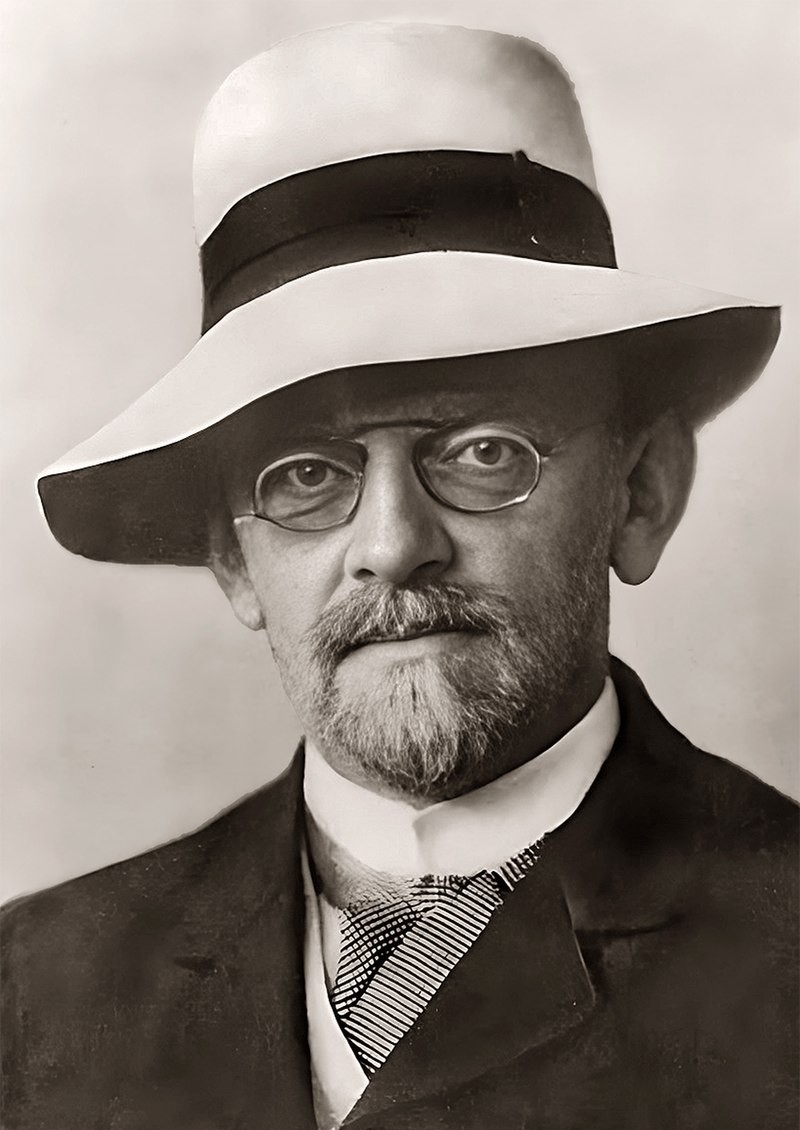
\includegraphics[width=.75\linewidth]{images/David_Hilbert}
									\caption{David Hilbert}
							\end{figure}
			\nextcolumn
							\begin{figure}
									\centering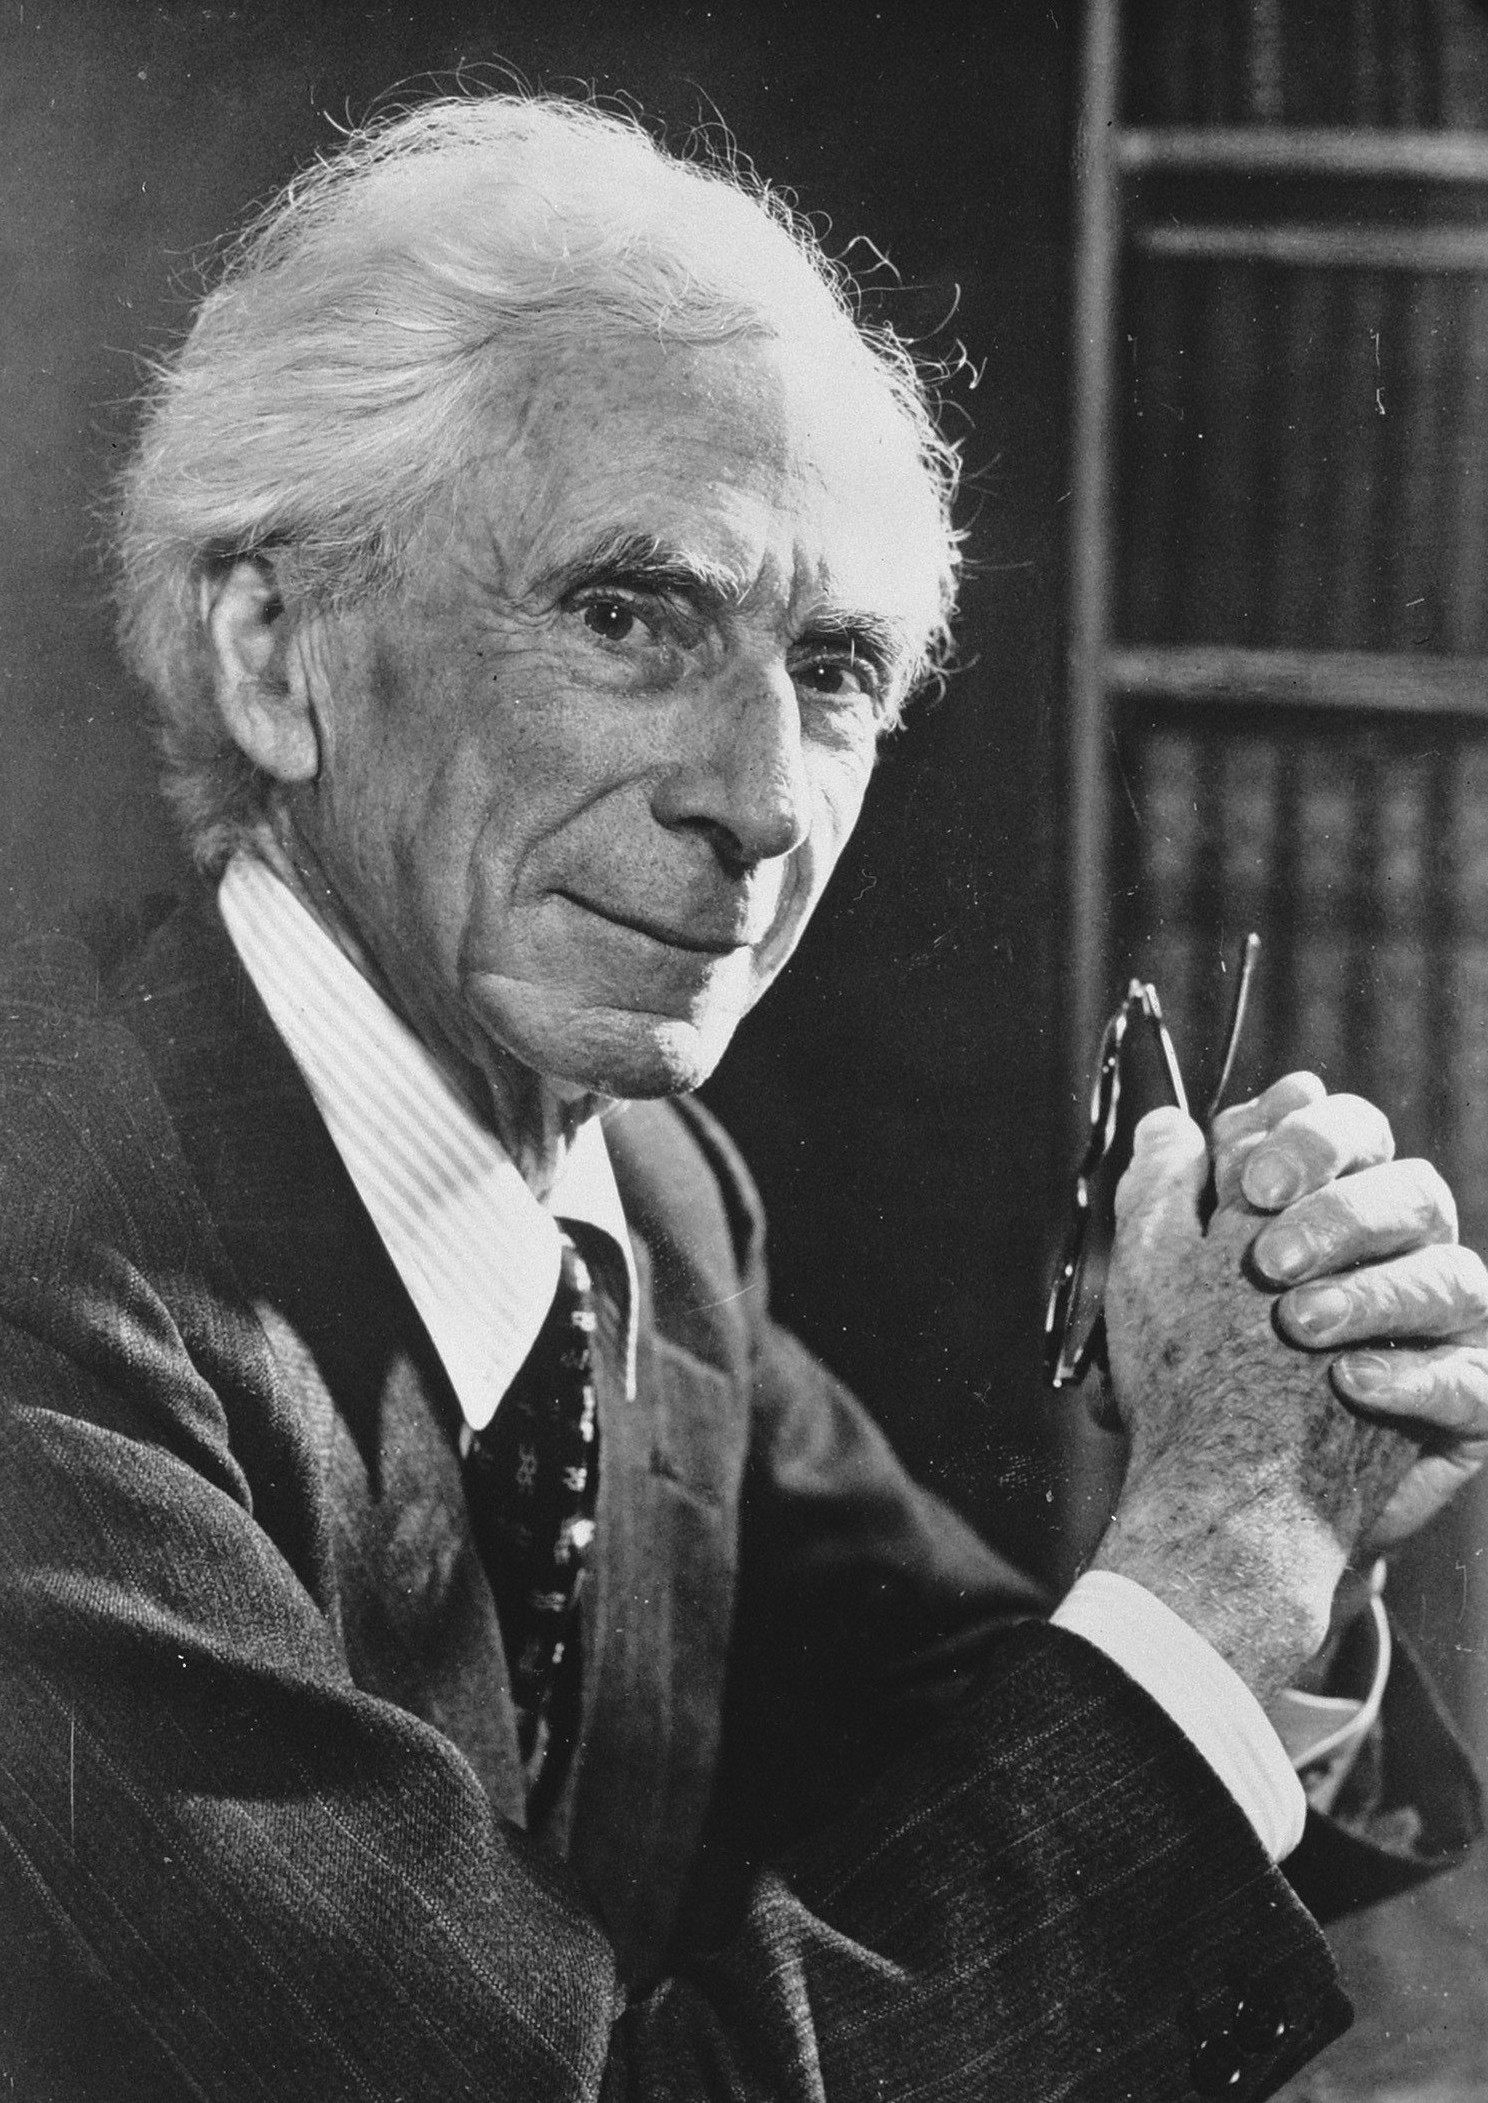
\includegraphics[width=.75\linewidth]{images/Bertrand_Russell}
									\caption{Bertrand Russell}
							\end{figure}
			\nextcolumn
							\begin{figure}
									\centering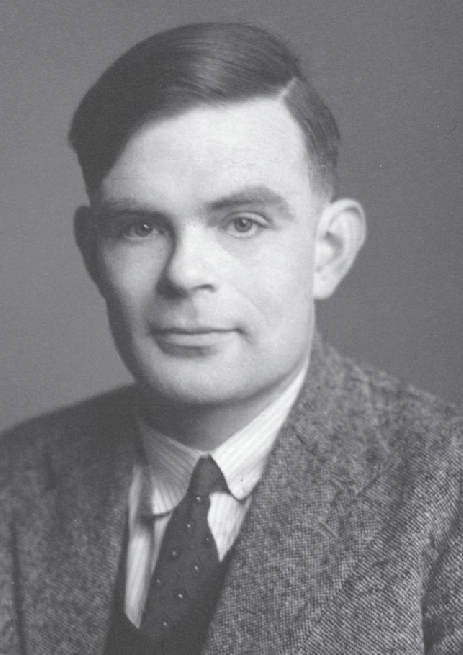
\includegraphics[width=.75\linewidth]{images/Alan_Turing}
									\caption{Alan Turing}
							\end{figure}
			\nextcolumn
							\begin{figure}
									\centering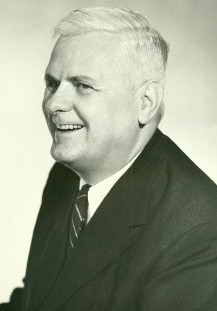
\includegraphics[width=.75\linewidth]{images/Alonzo_Church}
									\caption{Alonzo Church}
							\end{figure}
		\end{fancycolumns}
\end{frame}


\subsection{Revisiting the Simply Typed Lambda Calculus}
\begin{frame}{\insertsubsection}
		\begin{definition}{Syntax of Simply Typed Lambda Calculus}
				Recall the definition of the Lambda Calculus:
				\begin{equation}
						e ::= x \; | \; \lambda x.e \; | \; e \, e 
				\end{equation}
						Given a set of base types $B = \{b_1,b_2,...,b_N \}$ we define the type syntax
				\begin{equation}
								\tau ::= \tau \rightarrow \tau | T \text{, where } T \in B
				\end{equation}
		\end{definition}

		\pause 

		\begin{example}{Examples of Typed Lambda Terms}
				\begin{equation*}
								\lambda x : b_1 . x \text{ has type } b_1 \rightarrow b_1
				\end{equation*}

				\begin{equation*}
								\lambda x : b_1 . \lambda f : b_1 \rightarrow b_2 . f x \text{ has type } b_1 \rightarrow (b_1 \rightarrow b_2) \rightarrow b_2
				\end{equation*}

		\end{example}

\end{frame}

\begin{frame}{\insertsubsection}
		\begin{definition}{Typing Rules in the Simply Typed Lambda Calculus}
				We want to specify which lambda terms are well-typed by defining a relation between terms and types.
						\begin{itemize}
							\item{ A typing assumption has the form $x:b$, meaning variable $x$ has type $b$ }
							\item{ A typing context $\Gamma$ is a set of typing assumptions }
							\item{ A typing relation $\Gamma \vdash e:b$ indicates that $e$ has type $b$ in the typing context $\Gamma$}
							\item{ Typing assumptions in the typing context $\Gamma$ are assumed to be well-typed}
							\item{ Type assumptions outside the typing context are well-typed if they can be derived from the assumptions in the typing context $\Gamma$. }
						\end{itemize}

						\begin{fancycolumns}[columns=3,animation=none]
								\begin{equation}
												\frac{x:\sigma \in \Gamma}{\Gamma \vdash x:\sigma}
								\end{equation}
								\nextcolumn
								\begin{equation}
												\frac{\Gamma, x:\sigma \vdash e:\tau}{\Gamma \vdash (\lambda x: \sigma . e) : (\sigma \rightarrow \tau)}
								\end{equation}
								\nextcolumn
								\begin{equation}
												\frac{\Gamma \vdash e_1: \sigma \rightarrow \tau \;,\; \Gamma \vdash e_2:\sigma}{\Gamma \vdash e_1 \, e_2 : \tau}
								\end{equation}
						\end{fancycolumns}

		\end{definition}
\end{frame}

\subsection{The Curry-Howard Correspondance}
\begin{frame}{\insertsubsection}
		\begin{definition}{Empty and Nonempty Types}
				A type is called nonempty if there is a closed term of that type.
		\end{definition}
				\begin{example}{Types from our examples our nonempty}
				The types
				\begin{equation*}
						b_1 \rightarrow b_1, \; b_1 \rightarrow (b_1 \rightarrow b_2) \rightarrow b_2
				\end{equation*}
				are nonempty.
			\end{example}
		\begin{note}{Not all types are nonempty}
			Consider the type
			\begin{equation*}
					(b_1 \rightarrow b_2) \rightarrow b_1
			\end{equation*}
					Is it empty?
		\end{note}
\end{frame}

\begin{frame}{\insertsubsection}
		\begin{definition}{A Subset of Propositional Logic}
			We can construct a subset of propositional logic terms based on the following grammar:
			\begin{equation} 
							p ::= b \; | \;p \Rightarrow p
			\end{equation}
						\begin{fancycolumns}[columns=3,animation=none]
										\begin{equation}
												\frac{p \in \Gamma}{\Gamma \vdash p}
										\end{equation}
										\nextcolumn
										\begin{equation}
												\frac{\Gamma, p_1 \vdash p_2}{\Gamma \vdash p_1 \rightarrow p_2}
										\end{equation}
										\nextcolumn
										\begin{equation}
												\frac{\Gamma \vdash p_1, \; \Gamma \vdash p_1 \rightarrow p_2}{\Gamma \vdash p_2}
										\end{equation}
						\end{fancycolumns}
		\end{definition}

		\pause 

		\begin{note}{Comparison to Typing Rules}
						\begin{fancycolumns}[columns=3,animation=none]
										\begin{equation*}
												\frac{x:\sigma \in \Gamma}{\Gamma \vdash x:\sigma}
										\end{equation*}
										\nextcolumn
										\begin{equation*}
												\frac{\Gamma, x:\sigma \vdash e:\tau}{\Gamma \vdash (\lambda x: \sigma . e) : (\sigma \rightarrow \tau)}
										\end{equation*}
										\nextcolumn
										\begin{equation*}
												\frac{\Gamma \vdash e_1: \sigma \rightarrow \tau \;,\; \Gamma \vdash e_2:\sigma}{\Gamma \vdash e_1 \, e_2 : \tau}
										\end{equation*}
						\end{fancycolumns}
		\end{note}
\end{frame}

\begin{frame}{\insertsubsection}
		\begin{definition}{Curry-Howard Correspondance}
				\centering
				\begin{tabular}{|c|c|c|}
					\hline
								Algebra & Logic & (Haskell) Types \\
					\hline
					$a + b$     & $a \lor b$  & Either a b \\
					$a \cdot b$ & $a \land b$ & $(a,b)$ \\
					$a^b$ & $a \Rightarrow b$ & $a \rightarrow b$ \\
					$a=b$ & $a \Leftrightarrow b$ & $a$ isomorphic to $b$ \\
					$0$ & $ \top $ & Void \\
					$1$ & $ \perp $ & () \\
					\hline
				\end{tabular}
		\end{definition}
	
		\pause

		\begin{note}{Limitations of the Example}
		This is a simplified and incomplete representation of the correspondance between types in simply typed Lambda calculus and terms in propositional logic.
		\end{note}
\end{frame}


\subsection{Dependent Types}
\begin{frame}{\insertsubsection}
		\begin{note}{Implications of the Curry-Howard Correspondance}
						\begin{itemize}
								\item{The Curry-Howard Correspondance describes a correspondence between a given logic and a type system. }
								\item{For each proposition in the logic there is a corresponding non-empty type in the type system.}
								\item{For each proof of a given proposition, there is a program of the corresponding type.}
								\item{The correspondance applies not only to the simply-typed lambda calculus and propositional logic, but extends to more sophisticated logical calculi and type sytems (Girard-Reynolds, Hindley-Milner, ...).}
						\end{itemize}
		\end{note}
		\begin{definition}{Dependent Types}
						A dependent type is a type whose definition depends on a value.
		\end{definition}
\end{frame}

\begin{frame}{\insertsubsection}
		\begin{definition}{$\Pi$ Type}
					The $\Pi$ Type is the type of function whose type of return value depends on the value of its argument.
					\begin{equation*}
									\text{Notation: }\Pi_{x:A} B(x) \text{, where } A \text{ is a family of types and } B : A \rightarrow U \text{ is a family of types.}
					\end{equation*}
					$\Pi$ Types encode universal quantification: A function of type $\Pi_{x:A} B(x)$ assigns a type $B(a)$ to every $a \in A$
		\end{definition}

		\begin{example}{$\Pi$ Type}
						A function which maps natural numbers $n \in \mathbb{N}$ to $n$-tuples of floats has type $\Pi_{n: \mathbb{N}} \text{Vec}(\mathbb{R}, n)$.
		\end{example}

\end{frame}

\begin{frame}{\insertsubsection}
		\begin{definition}{$\Sigma$ Type}
						The $\Sigma$ Type is the type of a tuple in which the type of the second term depends on the value of the first term.
						\begin{equation*}
										\text{Notation: }\Sigma_{x:A} B(x) \text{, where } A \text{ is a family of types and } B : A \rightarrow U \text{ is a family of types.}
						\end{equation*}
						$\Sigma$ Types encode existential quantification: There is a $a \in A$ such that $B(a)$ is inhabited 
		\end{definition}
		\begin{example}{$\Sigma$ Type}
						A tuple consisting where the first term is a natural number and second term contains natural numbers greater than the value of the first term has type $\Sigma_{n: \mathbb{N}} \mathbb{N}_{>n}$.
		\end{example}
\end{frame}

\section{GADTs}

\subsection{From ADTs to GADTs}

\begin{slide}{\insertsubsection}

				\begin{note}{Warning: Compiler Extensions Required}
\begin{demo}
{-# LANGUAGE DataKinds       #-}
{-# LANGUAGE GADTs           #-}
{-# LANGUAGE RankNTypes      #-}
{-# LANGUAGE TypeFamilies    #-}
{-# LANGUAGE TypeOperators   #-}
\end{demo}
				\end{note}
\end{slide}


\begin{slide}{\insertsubsection}

\begin{lhsCode}{An Expression for Adding Integers}
\begin{code}
data ExprV1 = ExprV1 Int | AddV1 ExprV1 ExprV1
\end{code}
\end{lhsCode}

\pause

\begin{ghciOutput}{Kinds \& Types of Type and Data Constructors}
\begin{spec}
:k ExprV1
-- ExprV1 :: *
:t ExprV1 
-- ExprV1 :: Int -> ExprV1
:t AddV1
-- AddV1 :: ExprV1 -> ExprV1 -> ExprV1
\end{spec}
\end{ghciOutput}

\pause

\begin{lhsCode}{Evaluating our Expressions }
\begin{code}
evalExprV1 :: ExprV1 -> Int 
evalExprV1 (ExprV1 k) = k 
evalExprV1 (AddV1 e1 e2) = evalExprV1 e1 + evalExprV1 e2
\end{code}
\end{lhsCode}

\end{slide}


\begin{slide}{\insertsubsection}

\begin{lhsCode}{Extending Our Expression with Conditionals}
\begin{code}
data ExprV2 a where
  IntV2  :: Int -> ExprV2 Int
  BoolV2 :: Bool -> ExprV2 Bool
  AddV2 :: ExprV2 Int -> ExprV2 Int -> ExprV2 Int
  NotV2 :: ExprV2 Bool -> ExprV2 Bool
  IfV2 :: ExprV2 Bool -> ExprV2 a -> ExprV2 a -> ExprV2 a
\end{code}
\end{lhsCode}

\pause

\begin{ghciOutput}{Kinds \& Types of Type and Data Constructors}
\begin{spec}
:k ExprV2
-- ExprV2 :: * -> *
:t IntV2
-- IntV2 :: Int -> ExprV2 Int
:t AddV2
-- AddV2 :: ExprV2 Int -> ExprV2 Int
\end{spec}
\end{ghciOutput}

\end{slide}

\subsection{GADTs: Pattern Matching Leads to Type Refinement}

\begin{slide}{\insertsubsection}
\begin{lhsCode}{Evaluating our Extended Expressions }
\begin{code}
evalExprV2 :: ExprV2 a -> a
evalExprV2 (IntV2 i) = i
evalExprV2 (BoolV2 b) = b
evalExprV2 (AddV2 x y) = evalExprV2 x + evalExprV2 y
evalExprV2 (NotV2 x) = not $ evalExprV2 x
evalExprV2 (IfV2 c x y) = if evalExprV2 c 
                          then evalExprV2 x 
                          else evalExprV2 y
\end{code}
\end{lhsCode}
\end{slide}



\section{Dependently Typed Programming in Haskell}



\subsection{Lists are Unsafe}

\begin{slide}{\insertsubsection}

\begin{ghciOutput}{ Run-Time Errors }
\begin{spec}
head []
-- *** Exception: Prelude.head: empty list
maximum []
-- *** Exception: Prelude.head: empty list
["foo"] !! 1
-- *** Exception: Prelude.!!: index too large
\end{spec}
\end{ghciOutput}

\end{slide}


\subsection{GADTs Can Alleviate Some Problems}

\begin{slide}{\insertsubsection}

\begin{lhsCode}{ Nonempty Lists with GADTs }
\begin{code}
data ContainerStatus = Empty | NonEmpty

data SafeList :: * -> ContainerStatus -> * where
  Nil :: SafeList a Empty
  Cons :: a -> SafeList a b -> SafeList a NonEmpty

safeHead :: SafeList a NonEmpty -> a
safeHead (Cons x _) = x
\end{code}
\end{lhsCode}

\pause

\begin{ghciOutput}{Turning Run-Time into Compile-Time Errors}
\begin{spec}
safeHead $ Cons "bar" Nil
-- "bar"
safeHead $ Nil
-- error: Couldn't match type ‘Empty’ with ‘NonEmpty’
\end{spec}
\end{ghciOutput}

\end{slide}


\subsection{Fixed Length Vectors with Singleton Types}

\begin{slide}{\insertsubsection}


\begin{lhsCode}{Natural Numbers and Fixed Length Lists}
\begin{code}

data Nat where
  Zero :: Nat
  Succ :: Nat -> Nat

data Vec :: * -> Nat -> * where
  VNil :: Vec a 'Zero
  VCons :: a -> Vec a n -> Vec a ('Succ n)

\end{code}
\end{lhsCode}

\begin{ghciOutput}{Constructing Nats and Vecs}
\begin{spec}
Succ (Succ Zero) -- 2
VCons 2 (VCons 1 Nil) -- the vector [2, 1]
:t VCons 2 (VCons 1 VNil)
-- VCons 2 (VCons 1 VNil) :: Num a => Vec a ('Succ ('Succ 'Zero))
\end{spec}
\end{ghciOutput}


\end{slide}

\begin{slide}{\insertsubsection}

\begin{lhsCode}{A Safe Head Function}
\begin{code}

safeHead' :: Vec a ('Succ n) -> a
safeHead' (VCons x _) = x

\end{code}
\end{lhsCode}

\begin{ghciOutput}{Compile-Time Error}
\begin{spec}
safeHead' (VCons "foo" VNil)
-- "foo"
safeHead' VNil
-- error: Couldn't match type ‘'Zero’ with ‘'Succ n0’

\end{spec}
\end{ghciOutput}


\end{slide}

\begin{slide}{\insertsubsection}

\begin{lhsCode}{Comparing Nats (at Compile-Time!)}
\begin{code}
type family (m::Nat) :< (n::Nat) :: Bool
type instance m :< 'Zero = 'False
type instance Zero :< (Succ n) = 'True
type instance ('Succ m) :< (Succ n) = m :< n
\end{code}
\end{lhsCode}


\end{slide}


\begin{slide}{\insertsubsection}

\begin{note}{Safe Access (with Gaps)}
\begin{demo}

nth :: (m:<n) ~ 'True => --?-- -> Vec a n -> a
nth --?-- (VCons a _)        = a
nth --?-- (VCons _ as) = nth sm' as

\end{demo}
\end{note}

\pause

\begin{lhsCode}{Singleton Nats}
\begin{code}
data SNat :: Nat -> * where
  SZero :: SNat 'Zero
  -- SSucc :: forall (n::Nat).SNat n -> SNat ('Succ n)
  SSucc :: SNat n -> SNat ('Succ n)
\end{code}
\end{lhsCode}


\end{slide}




\begin{slide}{\insertsubsection}

\begin{lhsCode}{Safe Access}
\begin{code}

nth :: (m:<n) ~ 'True => SNat m -> Vec a n -> a
nth SZero (VCons a _)        = a
nth (SSucc sm') (VCons _ as) = nth sm' as

\end{code}
\end{lhsCode}

\begin{ghciOutput}{Compile-Time Error}
\begin{spec}
nth SZero (VCons "foo" VNil)
-- "foo"
nth (SSucc SZero) (VCons "foo" VNil)
-- error: Couldn't match type ‘'False’ with ‘'True’
\end{spec}
\end{ghciOutput}

\end{slide}

\begin{slide}{\insertsubsection}
				\begin{note}{Singleton Type Generation}
							\begin{figure}
									\centering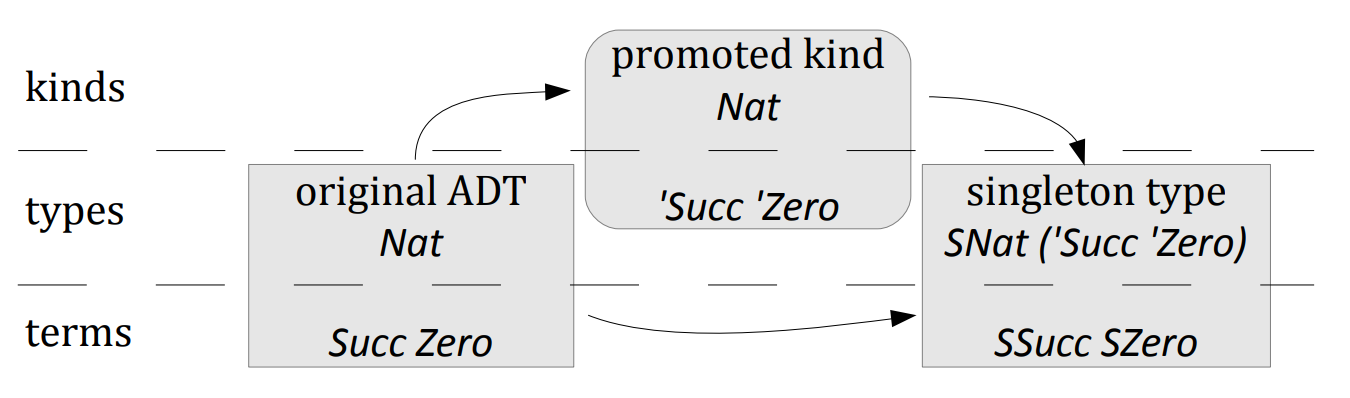
\includegraphics[width=.75\linewidth]{images/SingletonTypeGeneration}
											\caption{\textit{Eisenberg, R., \& Weirich, S. (2012). Dependently typed programming with singletons. In Proceedings of the 2012 Haskell Symposium (pp. 117–130). Association for Computing Machinery.}}
							\end{figure}
				\end{note}
\end{slide}


\subsection{Singleton Types - a Poor Man's Substitute for Dependent Types?}
\begin{slide}{\insertsubsection}
				\begin{definition}{What is a dependently typed language?}
								In a dependently typed language, types depend on run-time values.
				\end{definition}
				\begin{definition}{Is Haskell a dependently typed language?}
								Elements of a dependently typed language are supported by language extensions:
								\begin{itemize}
												\item{There is a  notion of type-level data with typing provided by DataKinds.}
												\item{We can use GADTs to create run-time representation of type-level data (using Singletons)}
								\end{itemize}
								Using Singletons oftentimes requires duplicate code for term- and type-level data. The \textit{Singletons} library can help to create this boilerplate code using \textit{Template Haskell}.
				\end{definition}
\end{slide}



%\subsection{Lists and Numbered Lists}
%\begin{frame}{\insertsubsection}
%	\begin{fancycolumns}
%		Lists can be nested to a depth of three:
%		\begin{itemize}
%			\item Item on the first level
%			\item Another item on the first level
%			\begin{itemize}
%				\item Item on the second level
%				\item Another item on the second level
%			\begin{itemize}
%			\item Item on the third level
%			\item Another item on the third level
%			\end{itemize}
%		\end{itemize}
%	\end{itemize}
%	\nextcolumn
%	Numbered lists can be nested to a depth of three:
%	\begin{enumerate}
%		\item Item on the first level
%		\item Another item on the first level
%		\begin{enumerate}
%			\item Item on the second level
%			\item Another item on the second level
%				\begin{enumerate}
%					\item Item on the third level
%					\item Another item on the third level
%				\end{enumerate}
%			\end{enumerate}
%		\end{enumerate}
%	\end{fancycolumns}
%\end{frame}
%
%%\subsection{Colored Boxes}
%\begin{frame}{\insertsubsection}
%	Normal versions:
%	\begin{fancycolumns}[columns=3]
%		\begin{definition}{A Definition}
%			This is a definition.
%		\end{definition}
%	\nextcolumn
%		\begin{example}{An {\color{blue} Example}}
%			This is an example.
%		\end{example}
%	\nextcolumn
%		\begin{note}{A {\color{red} Note}}
%			This is a note.
%		\end{note}
%	\end{fancycolumns}
%	\vfill
%	Versions without captions:
%	\begin{fancycolumns}[columns=3]
%		\begin{definition}{}
%			This is a {\color{orange} definition}.
%		\end{definition}
%	\nextcolumn
%		\begin{example}{}
%			This is an {\color{blue} example}.
%		\end{example}
%	\nextcolumn
%		\begin{note}{}
%			This is a {\color{red} note}.
%		\end{note}
%	\end{fancycolumns}
%	\vfill
%	Tight versions with white background (e.g., for use with pictures):
%	\begin{fancycolumns}[columns=3]
%		\begin{definitiontight}{A Definition}
%			\centering\includegraphics[width=.75\linewidth]{example-image}
%		\end{definitiontight}
%	\nextcolumn
%		\begin{exampletight}{An Example}
%			\centering\includegraphics[width=.75\linewidth]{example-image}
%		\end{exampletight}
%	\nextcolumn
%		\begin{notetight}{A Note}
%			\centering\includegraphics[width=.75\linewidth]{example-image}
%		\end{notetight}
%	\end{fancycolumns}
%\end{frame}
%
%{\MakeNewBox{amazing}{purple}
%\begin{frame}{Create New and Modify Existing Boxes}
%	\begin{fancycolumns}
%		\begin{amazing}{An Amazing Box}
%			You can create new boxes with \texttt{\textbackslash MakeNewBox\{name\}\{color\}} (which will check if any of the new box commands is already taken) or \texttt{\textbackslash DeclareBox\{name\}\{color\}} (which may overwrite existing commands). This box was created by \texttt{\textbackslash MakeNewBox\{amazing\}\{purple\}}.
%		\end{amazing}
%	\nextcolumn
%		{\UpdateBoxColor{definition}{teal}
%		\begin{definition}{This is a Definition}
%			With \texttt{\textbackslash UpdateBoxColor\{name\}\{color\}} you can change the color of a box (locally to the current group). This definition was changed with \texttt{\textbackslash UpdateBoxColor\{definition\}\{teal\}}.
%		\end{definition}}
%		\bigskip
%		\begin{definition}{Another Definition}
%			This definition appears outside of the group, so \texttt{\textbackslash UpdateBoxColor\{definition\}\{teal\}} is no longer active.
%		\end{definition}
%	\end{fancycolumns}
%\end{frame}
%}
%
%{\MakeNewBox[Improved-Box: ]{improved}{purple}[\hfill Jeah! \boxnumber]
%\begin{frame}{Counting Boxes!}
%	\UpdateBoxPrefix{definition}{Definition~\boxnumber: }%
%	\begin{definition}{Hey Look At My Number!}
%		With \texttt{\textbackslash UpdateBoxPrefix\{name\}\{prefix\}} you can change text to appear before the title of a box (locally to the current group). The macro \texttt{\textbackslash boxnumber} refers to the number of the current box that is robust against beamer overlays (but you do not have to use it).\medskip
%
%		This box was updated with \texttt{\textbackslash UpdateBoxPrefix\{definition\}\{Definition~\textbackslash boxnumber: \}}.
%		Similarly, there is \texttt{\textbackslash UpdateBoxSuffix\{name\}\{suffix\}} for text to appear after the title. As a comfort macro, there is \texttt{\textbackslash UpdateBoxSurround\{name\}\{prefix\}\{suffix\}}.
%	\end{definition}
%	\bigskip
%	\onslide<2->{\begin{improved}{This can be done at construction!}
%		Both \texttt{\textbackslash MakeNewBox[prefix]\{name\}\{color\}[postfix]} and \texttt{\textbackslash DeclareBox[prefix]\{name\}\{color\}[postfix]} have optional arguments that allow to set the prefix and suffix at construction. This box was created with \texttt{\textbackslash MakeNewBox[Improved-Box: ]\{improved\}\{purple\}[\textbackslash hfill Jeah! \textbackslash boxnumber]}.
%	\end{improved}}%
%\end{frame}
%}
%
%%\subsection{Advanced Management of Pictures}
%\begin{frame}{\insertsubsection}
%	\begin{fancycolumns}[t]
%		\begin{example}{\texttt{\textbackslash pic} command}
%			\centering\pic[width=0.5\textwidth,trim={.2\width} {.2\height} {.2\width} {.2\height},clip]{example-image}
%		\end{example}
%		\begin{note}{Explanation}
%			Using the command \texttt{\textbackslash pic\{filename\}} a picture can be included. It works like \texttt{\textbackslash adjincludegraphics} and therefore supports advanced options like \texttt{trim}.
%		\end{note}
%	\nextcolumn
%		\begin{example}{Automatic Links}
%			\centering\pic[width=0.5\textwidth]{example-image} % omit file extension of the image picture
%		\end{example}
%		\begin{note}{Explanation}
%			In order to automatically add a (source) link to the picture, the link simply has to be stored in a txt-file with the same filename.
%		\end{note}
%	\end{fancycolumns}
%\end{frame}
%
%%\subsection{Automatic Dark-Mode for Pictures}
%\begin{frame}{\insertsubsection}
%	\begin{fancycolumns}
%		\begin{notetight}{Normal Image with \texttt{\textbackslash pic}}
%			\centering
%			\pic[width=.7\textwidth]{example-image}
%		\end{notetight}
%	\nextcolumn
%		\begin{notetight}{Inverted Image with \texttt{\textbackslash picDark} (in dark-mode only)}
%			\centering
%			\picDark[width=.7\textwidth]{example-image.jpg} % does only work for bitmap images so far
%		\end{notetight}
%	\end{fancycolumns}
%	\begin{note}{Explanation}
%		Using \texttt{\textbackslash picDark} instead of \texttt{\textbackslash pic}, the dark version of an image that is saved as \texttt{<image-name>-dark} automatically gets used when dark-mode is enabled.
%
%		Images can also automatically be inverted if there is no separate dark version. Therefore, white gets converted to a dark gray that matches the dark background color of the slides.
%	\end{note}
%\end{frame}
%
%%\section{Slide Layouts}
%
%%\subsection{Multiple Columns}
%\begin{frame}{\insertsubsection}
%	\begin{fancycolumns}[columns=4] % default: 2 columns
%		This is an example text that is shown in the \textbf{first column}.
%	\nextcolumn
%		This is an example text that is shown in the \textbf{second column}.
%	\nextcolumn
%		This is an example text that is shown in the \textbf{third column}.
%	\nextcolumn
%		This is an example text that is shown in the \textbf{last column}.
%	\end{fancycolumns}
%	\vfill
%	\begin{note}{Explanation}
%		Columns are separated by the command \texttt{\textbackslash nextcolumn}.
%
%		The option \texttt{columns} specifies the number of columns that should be generated. The default number of columns is two.
%	\end{note}
%\end{frame}
%
%%\subsection{Columns with Custom Width}
%\begin{frame}{\insertsubsection}
%	\begin{fancycolumns}[columns=3,widths={20,30}]
%		\begin{example}{}
%			The \textbf{first column} takes 20\,\% of the width of the slide.
%		\end{example}
%	\nextcolumn
%		\begin{example}{}
%			The \textbf{second column} takes 30\,\% of the width of the slide.
%		\end{example}
%	\nextcolumn
%		\begin{example}{}
%			The \textbf{third column} takes the remaining 50\,\% of the width of the slide.
%		\end{example}
%	\end{fancycolumns}
%	\vfill
%	\begin{note}{Explanation}
%		The widths of the single columns can also be manually specified by a list of percentages given to the option \texttt{widths}.
%
%		All columns whose width is not specified are equally split over the remaining space.
%	\end{note}
%\end{frame}
%
%%\subsection{Columns with Custom Height}
%\begin{frame}{\insertsubsection}
%	\begin{fancycolumns}[height=6cm]
%		\begin{example}{}
%			This is the content of the first column.
%		\end{example}
%		\begin{note}{Explanation}
%			If the content of a column exceeds a certain height, the common centering of all columns will not work anymore because beamer does not define the height of a slide. In this case, you can set the height of the columns manually by adding the option \texttt{height=<height>}.
%		\end{note}
%	\nextcolumn
%		\begin{example}{}
%			This is the content of the second column. It is too high and would make the first column move downwards without additional options.
%			\vspace{80mm}
%		\end{example}
%	\end{fancycolumns}
%\end{frame}
%
%%\subsection{Nested Columns}
%\begin{frame}{\insertsubsection}
%	\begin{fancycolumns}[T]
%		\begin{example}{}
%			This is the content of the first column.
%		\end{example}
%		\begin{fancycolumns}[columns=4]
%			\mynote{}{1.1}
%			\nextcolumn
%			\mynote{}{1.2}
%			\nextcolumn
%			\mynote{}{1.3}
%			\nextcolumn
%			\mynote{}{1.4}
%		\end{fancycolumns}
%	\nextcolumn
%		\begin{example}{}
%			A column on the right side
%		\end{example}
%		\begin{fancycolumns}[T]
%			\mynote{}{2.1}
%			\begin{fancycolumns}[columns=3]
%				\mynote{}{2.1.1}
%				\nextcolumn
%				\mynote{}{2.1.2}
%				\nextcolumn
%				\mynote{}{2.1.3}
%			\end{fancycolumns}
%			\nextcolumn
%			\mynote{}{2.2}
%		\end{fancycolumns}
%	\end{fancycolumns}
%\end{frame}
%
%%\subsection{Column Animations}
%\begin{frame}{\insertsubsection\ -- Option keep}
%	\begin{fancycolumns}[columns=3,keep] % short for animation=keep
%		This is an example text that is shown in the \textbf{first column}.
%	\nextcolumn
%		This is an example text that is shown in the \textbf{second column}.
%	\nextcolumn
%		This is an example text that is shown in the \textbf{third column}.
%	\end{fancycolumns}
%	\vfill
%	\begin{note}{Explanation}
%		The option \texttt{keep} (short for \texttt{animation=keep}) introduces an animation which lets the columns appear one after another.
%
%		The previous columns are kept on the slide when a new column is displayed.
%
%		Animations are ignored in handout mode.
%	\end{note}
%\end{frame}
%
%\begin{frame}{\insertsubsection\ -- Option forget}
%	\begin{fancycolumns}[columns=3,forget] % short for animation=forget
%		This is an example text that is shown in the \textbf{first column}.
%	\nextcolumn
%		This is an example text that is shown in the \textbf{second column}.
%	\nextcolumn
%		This is an example text that is shown in the \textbf{third column}.
%	\end{fancycolumns}
%	\vfill
%	\begin{note}{Explanation}
%		The option \texttt{forget} (short for \texttt{animation=forget}) introduces an animation which lets the columns appear one after another.
%
%		The previous columns are removed when a new column is displayed.
%
%		Animations are ignored in handout mode.
%	\end{note}
%\end{frame}
%
%\begin{frame}{\insertsubsection\ -- Option animation=none}
%	\begin{fancycolumns}[columns=3,animation=none]
%		This is an example text that is shown in the \textbf{first column}.
%	\nextcolumn
%		This is an example text that is shown in the \textbf{second column}.
%	\nextcolumn
%		This is an example text that is shown in the \textbf{third column}.
%	\end{fancycolumns}
%	\vfill
%	\begin{note}{Explanation}
%		The option \texttt{animation=none} deactivates the animation of the columns.
%
%		In the template, this is the default. However, you can overwrite the defaults to animate all slides easily (see \texttt{setfancycolumnsdefault} in the source code). Then, it might be necessary to deactivate those animations for some slides.
%	\end{note}
%\end{frame}
%
%\begin{frame}[label=current]{\insertsubsection\ -- Option reverse}
%	\begin{fancycolumns}[columns=3,forget,reverse]
%		This is an example text that is shown in the \textbf{first column}.
%	\nextcolumn
%		This is an example text that is shown in the \textbf{second column}.
%	\nextcolumn
%		This is an example text that is shown in the \textbf{third column}.
%	\end{fancycolumns}
%	\vfill
%	\begin{note}{Explanation}
%		The option \texttt{reverse} inverts the order of any animation that is specified (i.e., using \texttt{keep} or \texttt{forget}).
%	\end{note}
%\end{frame}
%
%%\section{Other Features}
%
%%\subsection{Auto-Scaling for Long Titles}
%\begin{frame}{\insertsubsection\ -- Long Titles are Scaled Down to the Available Space}
%	\begin{note}{Explanation}
%		Very long frame titles are scaled down automatically.
%
%		\hfill\hfill\hfill This can avoid annoying linebreaks for a single character or word.\hfill~
%
%		\hfill Use with care.
%	\end{note}
%\end{frame}
%
%%\subsection{Easy Navigation in Slides}
%\begin{frame}{\insertsubsection}
%	\vfill
%	Click on the title (here \textbf{\insertshorttitle}) or subtitle (here \textbf{\insertshortsubtitle}) in the slide footer to jump to the title slide.
%	\vfill
%	Click on the section title (here \textbf{\insertsection}) in the slide footer to jump to the section overview.
%	\vfill
%	In the section overview, click on sections or subsections to jump to another part.
%	\vfill
%\end{frame}
%
%\subsection{Repeating the Last Title Slide}
 % can be used as the last slide of your talk
\againtitle

%\subsection{Content Overview}
% helpful to navigate to specific content, no need to show during the talk
%\contentoverview % create a content overview with one column
%\contentoverview[3] % create a content overview with three columns

\end{document}
